\documentclass[12pt,a4paper]{article}

\usepackage{fontspec}
\usepackage{polyglossia}
\setdefaultlanguage{ukrainian}
\setmainfont{Times New Roman}
\newfontfamily\cyrillicfonttt{Times New Roman}

\usepackage{amsmath,amssymb}
\usepackage{geometry}
\usepackage{graphicx}
\usepackage{float}
\usepackage{caption}
\usepackage{setspace}

\geometry{left=25mm,right=15mm,top=20mm,bottom=20mm}
\setstretch{1.2}
\captionsetup{justification=centering}

\begin{document}

\begin{titlepage}
    \begin{center}
        \textbf{Київський національний університет імені Тараса Шевченка}\\
        \textbf{Факультет комп'ютерних наук та кібернетики}
    \end{center}

    \vspace{4cm}

    \begin{center}
        \textbf{\Large ЗВІТ}\\
        \vspace{0.5cm}
        \textbf{\large до лабораторної роботи №\,2}\\
        \vspace{0.5cm}
        з дисципліни \textit{«Основи нелінійної динаміки»}\\
        \vspace{0.7cm}
        \textbf{Тема: Фазові портрети нелінійних систем\\(метод лінеаризації в околі особливих точок)}
    \end{center}

    \vfill

    \begin{flushright}
        Виконав:\\
        Кіщук Ярослав Ярославович
    \end{flushright}

    \vspace{1.5cm}

    \begin{center}
        Київ --- 2026
    \end{center}
\end{titlepage}

\tableofcontents
\newpage

\section{Завдання 3.7}

\subsection{Запис системи}

Розглянемо автономну систему звичайних диференціальних рівнянь другого порядку на площині:
\begin{equation}\label{eq:system}
\begin{cases}
\dot{x} = P(x,y) = (2x-y)(x-2),\\
\dot{y} = Q(x,y) = xy - 2.
\end{cases}
\end{equation}
На рисунках показано фазові траєкторії, поле напрямків та допоміжні криві $\dot{x}=0$, $\dot{y}=0$.

\subsection{Знаходження особливих точок}

Особливі точки системи~\eqref{eq:system} --- розв'язки системи алгебраїчних рівнянь
\begin{equation*}
P(x,y)=0,\qquad Q(x,y)=0.
\end{equation*}
З умови $Q(x,y)= xy-2 = 0$ маємо при $x\neq 0$ зв'язок $y=\dfrac{2}{x}$.
Підстановка у $P=0$:
\begin{equation*}
(2x-y)(x-2)=0 \quad \Rightarrow \quad \bigl(2x-\tfrac{2}{x}\bigr)(x-2)=0.
\end{equation*}
Якщо $x=2$, то з $xy=2$ одержуємо $y=1$, тобто точка $M_1(2,1)$.
Якщо $2x-\dfrac{2}{x}=0$, тобто $x^2=1$, то $x=\pm 1$, а $y=\dfrac{2}{x}$ дає точки $M_2(1,2)$ та $M_3(-1,-2)$.

\textbf{Результат:} особливі точки системи~\eqref{eq:system}
\begin{equation*}
M_1(2,1),\qquad M_2(1,2),\qquad M_3(-1,-2).
\end{equation*}

\subsection{Матриця Якобі та інваріанти лінеаризації}

Частинні похідні:
$P'_x=\dfrac{\partial P}{\partial x}$, $P'_y=\dfrac{\partial P}{\partial y}$,
$Q'_x=\dfrac{\partial Q}{\partial x}$, $Q'_y=\dfrac{\partial Q}{\partial y}$.
Для системи~\eqref{eq:system} обчислення дає
\begin{align*}
P'_x(x,y) &= 4x-y-4,\qquad P'_y(x,y) = 2-x,\\
Q'_x(x,y) &= y,\qquad Q'_y(x,y) = x.
\end{align*}
Матриця Якобі має вигляд
\begin{equation}\label{eq:jacobian}
J(x,y)=
\begin{pmatrix}
P'_x(x,y) & P'_y(x,y)\\
Q'_x(x,y) & Q'_y(x,y)
\end{pmatrix}
=
\begin{pmatrix}
4x-y-4 & 2-x\\
y & x
\end{pmatrix}.
\end{equation}

Визначник і слід матриці Якобі в точці $(x_0,y_0)$:
\begin{equation*}
\Delta(x_0,y_0)=
\begin{vmatrix}
P'_x(x_0,y_0) & P'_y(x_0,y_0)\\
Q'_x(x_0,y_0) & Q'_y(x_0,y_0)
\end{vmatrix},
\qquad
\sigma(x_0,y_0)=P'_x(x_0,y_0)+Q'_y(x_0,y_0).
\end{equation*}
Для системи~\eqref{eq:system}:
\begin{equation*}
\Delta(x,y)=P'_x Q'_y-P'_y Q'_x=(4x-y-4)x-(2-x)y,\qquad
\sigma(x,y)=P'_x+Q'_y=5x-y-4.
\end{equation*}

Розкладемо $P,Q$ у ряд Тейлора в околі особливої точки $(x_0,y_0)$. Після позначення
\begin{equation*}
P'_x(x_0,y_0)=a_0,\quad P'_y(x_0,y_0)=b_0,\quad Q'_x(x_0,y_0)=c_0,\quad Q'_y(x_0,y_0)=d_0
\end{equation*}
система набуває вигляду
\begin{equation*}
\begin{aligned}
\dot{x} &= a_0(x-x_0)+b_0(y-y_0)+R_1(x,y),\\
\dot{y} &= c_0(x-x_0)+d_0(y-y_0)+R_2(x,y),
\end{aligned}
\end{equation*}
де функції $R_1(x,y)$, $R_2(x,y)$ --- наближення вищого порядку.

Паралельним перенесенням особливої точки в початок координат $x=x_0+\xi$, $y=y_0+\eta$ отримуємо систему
\begin{equation*}
\dot{\xi}=a_0\xi+b_0\eta+\tilde{R}_1(\xi,\eta),\qquad
\dot{\eta}=c_0\xi+d_0\eta+\tilde{R}_2(\xi,\eta).
\end{equation*}
Відкидаючи нелінійні члени, отримуємо лінеаризовану систему
\begin{equation*}
\begin{pmatrix}\dot{\xi}\\ \dot{\eta}\end{pmatrix}
=
\begin{pmatrix}a_0 & b_0\\ c_0 & d_0\end{pmatrix}
\begin{pmatrix}\xi\\ \eta\end{pmatrix}
= J(x_0,y_0)\begin{pmatrix}\xi\\ \eta\end{pmatrix}.
\end{equation*}
За теоремою Ляпунова про лінійне наближення, якщо матриця $J(x_0,y_0)$ не має суто уявних або нульових власних чисел, то в достатньо малому $\delta$-околі $U_\delta(x_0,y_0)$ локальні фазові портрети вихідної нелінійної системи та лінеаризованої системи
$\dot{\xi}=a_0\xi+b_0\eta$, $\dot{\eta}=c_0\xi+d_0\eta$ є топологічно еквівалентними.
Характеристичне рівняння --- $\det(J(x_0,y_0)-\lambda I)=0$.

\subsection{Лінеаризація в околі $M_1(2,1)$}\label{subsec:M1_37}

Підставляючи $(x,y)=(2,1)$ у~\eqref{eq:jacobian}, одержуємо
\begin{equation*}
J(M_1)=X
\begin{pmatrix}
3 & 0\\
1 & 2
\end{pmatrix}.
\end{equation*}
Характеристичне рівняння:
\begin{equation*}
\det(J(M_1)-\lambda I)=(3-\lambda)(2-\lambda)=\lambda^2-5\lambda+6=0,
\end{equation*}
звідки $\lambda_1=3$, $\lambda_2=2$.
Обидва корені дійсні, додатні та різні: відповідне положення рівноваги лінеаризованої системи є \textbf{нестійким вузлом}.
Маємо $\sigma(2,1)=5$, $\Delta(2,1)=6\neq 0$; точка $M_1$ --- проста.
Оскільки $\lambda_1,\lambda_2$ дійсні та ненульові, виконана умова теореми Ляпунова про лінійне наближення: локальний фазовий портрет вихідної системи в околі $M_1$ топологічно еквівалентний лінеаризованій системі.

Власні вектори шукаємо у вигляді $s=(\alpha,\beta)^T$ з рівняння $(J-\lambda I)s=0$:
\begin{itemize}
    \item для $\lambda_1=3$: $\begin{pmatrix}0&0\\1&-1\end{pmatrix}\begin{pmatrix}\alpha\\ \beta\end{pmatrix}=0$ дає $\alpha-\beta=0$, тобто $\alpha=\beta$; беремо $\alpha=1,\beta=1$, звідки $s^{(1)}=(1,1)^T$;
    \item для $\lambda_2=2$: $\begin{pmatrix}1&0\\1&0\end{pmatrix}\begin{pmatrix}\alpha\\ \beta\end{pmatrix}=0$ дає $\alpha=0$, $\beta$ --- довільне; беремо $\alpha=0,\beta=1$, звідки $s^{(2)}=(0,1)^T$.
\end{itemize}

\paragraph{Геометрія вузла.}
Загальний розв'язок лінеаризованої системи в координатах $\xi=x-2$, $\eta=y-1$:
\begin{equation*}
\begin{pmatrix}\xi(t)\\ \eta(t)\end{pmatrix}
= C_1\,e^{3t}\begin{pmatrix}1\\1\end{pmatrix}
+ C_2\,e^{2t}\begin{pmatrix}0\\1\end{pmatrix}.
\end{equation*}
Менше за модулем власне число --- $\lambda_2=2$ з \emph{«повільною»} модою та вектором $s^{(2)}=(0,1)^T$; більше --- $\lambda_1=3$ з \emph{«швидкою»} модою і $s^{(1)}=(1,1)^T$.
Поблизу $M_1$ (малі $|t-t_0|$) в експонентах домінує повільна мода, тому \textbf{усі траєкторії виходять з $M_1$ майже дотично до $s^{(2)}=(0,1)^T$} (вертикально); далеко від точки переважає швидка мода, тому «хвости» траєкторій вирівнюються уздовж $s^{(1)}=(1,1)^T$.
Відношення характеристичних швидкостей $|\lambda_1|/|\lambda_2|=3/2=1{,}5$ невелике --- вузол \textbf{помірно витягнутий} уздовж $s^{(2)}$.

\begin{figure}[H]
    \centering
    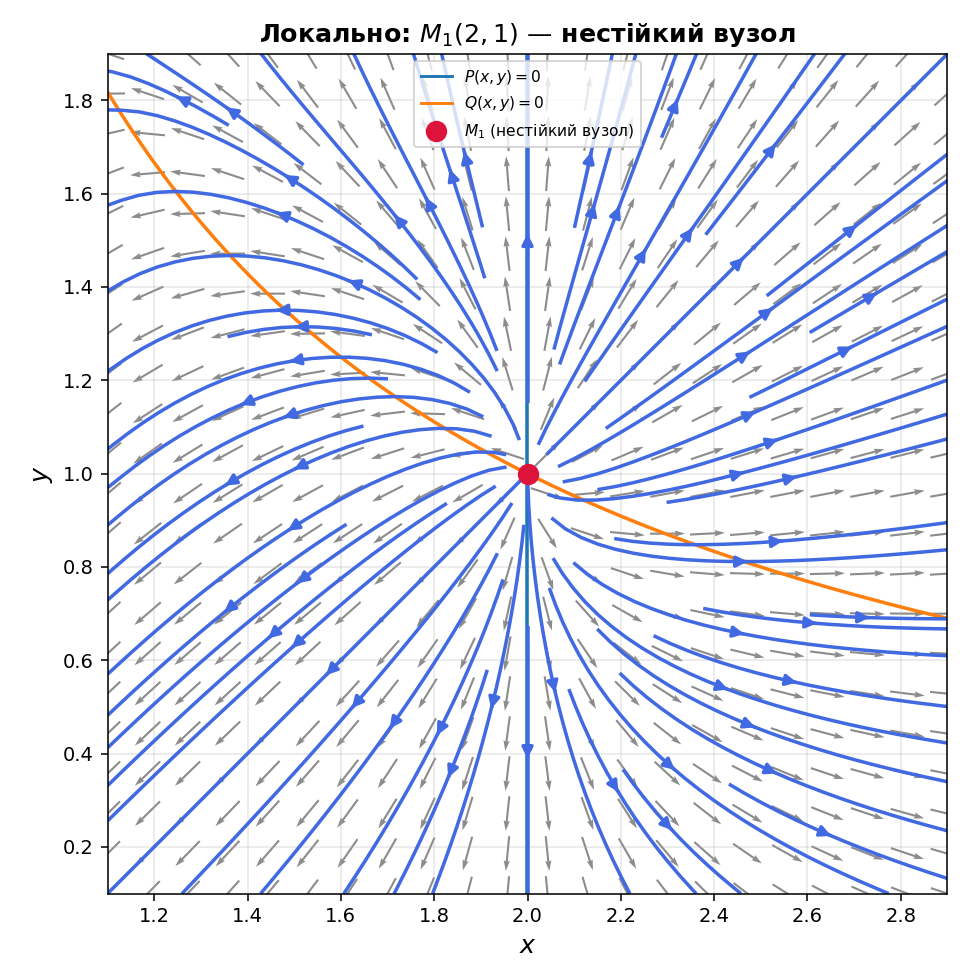
\includegraphics[width=0.72\textwidth]{local_M1.png}
    \caption{Локальний портрет: траєкторії, поле напрямків, криві $\dot{x}=0$ та $\dot{y}=0$; $M_1(2,1)$ --- нестійкий вузол}
\end{figure}

\paragraph{Код побудови (Python).}
\begin{verbatim}
plot_local(M1, "M1",
    r"Локально: $M_1(2,1)$ — нестійкий вузол")

def plot_local(center, tag, title, density=1.55):
    span = 0.9
    xlim = (center[0] - span, center[0] + span)
    ylim = (center[1] - span, center[1] + span)
    fig, ax = plt.subplots(figsize=(7, 7), dpi=140)
    plot_base(ax, xlim, ylim, quiver_n=22)
    # plot_dx_dy_zero_curves: криві P=0 (dx/dt=0) та Q=0 (dy/dt=0)
    plot_dx_dy_zero_curves(ax, xlim, ylim)
    seeds = make_seed_grid(xlim, ylim, n=11,
        avoid=[(M1,0.12), (M2,0.12), (M3,0.12)])
    extra = [
        [xlim[0]+0.05, ylim[0]+0.05], [xlim[1]-0.05, ylim[1]-0.05],
        [xlim[0]+0.05, ylim[1]-0.05], [xlim[1]-0.05, ylim[0]+0.05]]
    seeds = np.vstack([seeds, np.array(extra)])
    stream_on_ax(ax, xlim, ylim, density=density, seeds=seeds)
    mark_equilibria(ax)
    ax.set_title(title)
    fig.savefig(f"local_{tag}.png")
    plt.close(fig)
\end{verbatim}

\subsection{Лінеаризація в околі $M_2(1,2)$}

\begin{equation*}
J(M_2)=
\begin{pmatrix}
-2 & 1\\
2 & 1
\end{pmatrix}.
\end{equation*}
Характеристичне рівняння:
\begin{equation*}
\begin{vmatrix}
-2-\lambda & 1\\
2 & 1-\lambda
\end{vmatrix}
=\lambda^2+\lambda-4=0,
\end{equation*}
\begin{equation*}
\lambda_{1,2}=\frac{-1\pm\sqrt{17}}{2}\approx 1{,}56,\;\; -2{,}56.
\end{equation*}
Корені дійсні різних знаків --- \textbf{сідло}. Тут $\sigma(1,2)=-1$, $\Delta(1,2)=-4\neq 0$.
Оскільки $\lambda_{1,2}$ дійсні та ненульові, виконана умова теореми Ляпунова про лінійне наближення: локальний портрет вихідної системи в околі $M_2$ топологічно еквівалентний лінеаризованій системі.

Власні напрямки шукаємо у вигляді $s=(\alpha,\beta)^T$ з рівняння $(J-\lambda I)s=0$: з першого рядка $(-2-\lambda)\alpha+\beta=0$, покладемо $\alpha=1$, тоді $\beta=2+\lambda$.
Тобто для $\lambda_+=\dfrac{-1+\sqrt{17}}{2}$ маємо власний вектор $s_+=(1,\;2+\lambda_+)^T$, для $\lambda_-=\dfrac{-1-\sqrt{17}}{2}$ --- $s_-=(1,\;2+\lambda_-)^T$.
У координатах $(x,y)$ сепаратриси лінеаризації мають рівняння прямих через $M_2$ із нахилами $k_\pm = 2+\lambda_\pm = \dfrac{3\pm\sqrt{17}}{2}$.

Напрямок руху на сепаратрисах визначаємо підстановкою пробної точки, яка дещо зміщена від $M_2$ уздовж відповідного власного напрямку, у праві частини системи~\eqref{eq:system}.

Для $\lambda_+\approx 1{,}56$ маємо $s_+=(1,\;(3+\sqrt{17})/2)\approx(1;\,3{,}56)$. Візьмемо малий зсув $\varepsilon=0{,}1$ уздовж $s_+$:
\begin{equation*}
(x,y)=M_2+\varepsilon\,s_+\approx(1{,}1;\;2{,}356).
\end{equation*}
Підставляючи у~\eqref{eq:system}:
\begin{align*}
\dot x &= P(1{,}1;\,2{,}356)=(2{\cdot}1{,}1-2{,}356)(1{,}1-2)\approx(-0{,}156)(-0{,}9)\approx 0{,}14>0,\\
\dot y &= Q(1{,}1;\,2{,}356)=1{,}1{\cdot}2{,}356-2\approx 0{,}59>0.
\end{align*}
Вектор $(\dot x,\dot y)$ у цій точці напрямлений «вправо-вгору» --- тобто від $M_2$. Це підтверджує, що $s_+$ --- нестійкий напрямок сідла (траєкторія віддаляється від $M_2$).

Для $\lambda_-\approx -2{,}56$ маємо $s_-=(1,\;(3-\sqrt{17})/2)\approx(1;\,-0{,}56)$. Аналогічно, при $\varepsilon=0{,}1$ пробна точка $M_2+\varepsilon s_-\approx(1{,}1;\,1{,}944)$ дає
\begin{equation*}
\dot x\approx-0{,}23<0,\qquad \dot y\approx 0{,}14>0,
\end{equation*}
тобто вектор $(\dot x,\dot y)$ напрямлений у бік $M_2(1,2)$ --- отже, $s_-$ --- стійкий напрямок (траєкторія наближається до $M_2$).

\begin{figure}[H]
    \centering
    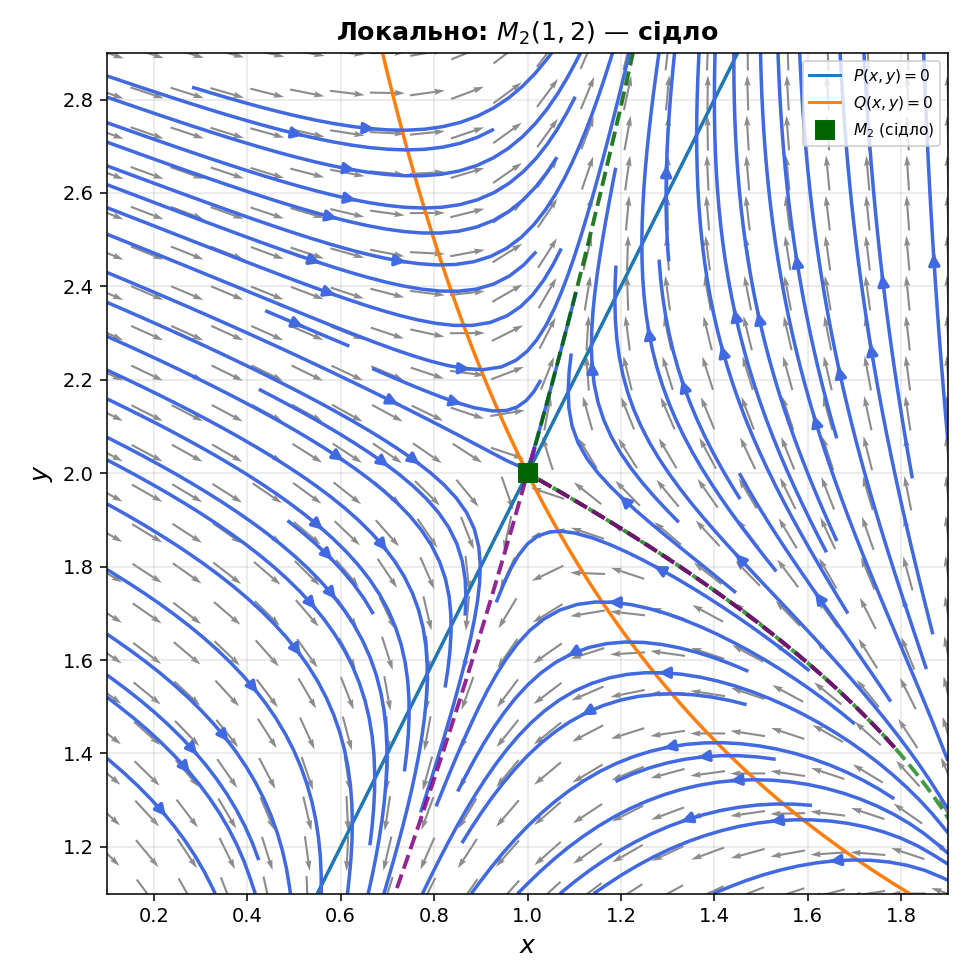
\includegraphics[width=0.72\textwidth]{local_M2.png}
    \caption{Локально біля $M_2(1,2)$ (сідло): траєкторії, поле напрямків, криві $\dot{x}=0$, $\dot{y}=0$, сепаратриси}
\end{figure}

\paragraph{Код побудови (Python).}
Виклик \texttt{plot\_local(M2, "M2", ...)}. Усередині \texttt{plot\_local} після \texttt{stream\_on\_ax}:
\begin{verbatim}
if np.allclose(center, M2):
    saddle_separatrices_plot(ax, eps=0.018, t_max=5.0)

def saddle_separatrices_plot(ax, eps=0.02, t_max=8.0):
    starts = []
    for sgn in (-1.0, 1.0):
        starts.append(M2 + sgn * eps * v_unstable)
        starts.append(M2 + sgn * eps * v_stable)
    for (x0, y0) in starts:
        for t_span in ((0.0, t_max), (0.0, -t_max)):
            xs, ys = integrate_separatrix(x0, y0, t_span)
            ax.plot(xs, ys, "--", linewidth=2.0)
\end{verbatim}

\subsection{Лінеаризація в околі $M_3(-1,-2)$}

\begin{equation*}
J(M_3)=
\begin{pmatrix}
-6 & 3\\
-2 & -1
\end{pmatrix}.
\end{equation*}
Характеристичне рівняння:
\begin{equation*}
\lambda^2+7\lambda+12=0,\qquad \lambda_1=-3,\quad \lambda_2=-4.
\end{equation*}
Обидва корені дійсні від'ємні --- \textbf{стійкий вузол}. Маємо $\sigma(-1,-2)=-7$, $\Delta(-1,-2)=12\neq 0$.
Оскільки $\lambda_1,\lambda_2$ дійсні та ненульові, виконана умова теореми Ляпунова про лінійне наближення: локальний портрет вихідної системи в околі $M_3$ топологічно еквівалентний лінеаризованій системі.

Власні вектори шукаємо у вигляді $s=(\alpha,\beta)^T$ з рівняння $(J-\lambda I)s=0$:
\begin{itemize}
    \item для $\lambda=-3$: перший рядок $(J+3I)s=0$ дає $-3\alpha+3\beta=0$, тобто $\alpha=\beta$; беремо $\alpha=1,\beta=1$, звідки $s^{(1)}=(1,1)^T$;
    \item для $\lambda=-4$: перший рядок $(J+4I)s=0$ дає $-2\alpha+3\beta=0$, тобто $\beta=\tfrac{2}{3}\alpha$; беремо $\alpha=3,\beta=2$, звідки $s^{(2)}=(3,2)^T$.
\end{itemize}

\paragraph{Геометрія вузла.}
Загальний розв'язок лінеаризованої системи в координатах $\xi=x+1$, $\eta=y+2$:
\begin{equation*}
\begin{pmatrix}\xi(t)\\ \eta(t)\end{pmatrix}
= C_1\,e^{-3t}\begin{pmatrix}1\\1\end{pmatrix}
+ C_2\,e^{-4t}\begin{pmatrix}3\\2\end{pmatrix}.
\end{equation*}
Менше за модулем власне число --- $\lambda_1=-3$ з \emph{«повільною»} модою та вектором $s^{(1)}=(1,1)^T$ (нахил $1$); більше --- $\lambda_2=-4$ з \emph{«швидкою»} модою і $s^{(2)}=(3,2)^T$ (нахил $2/3$).
При $t\to+\infty$ швидша експонента $e^{-4t}$ згасає першою, тому \textbf{всі траєкторії входять у $M_3$ майже дотично до $s^{(1)}$}; далеко від точки домінує «швидка» мода, тому хвости траєкторій тягнуться уздовж $s^{(2)}$.
Відношення $|\lambda_2|/|\lambda_1|=4/3\approx 1{,}33$ --- невелике, тож вузол \textbf{трохи витягнутий} уздовж $s^{(1)}$ (що і видно на рисунку).

\begin{figure}[H]
    \centering
    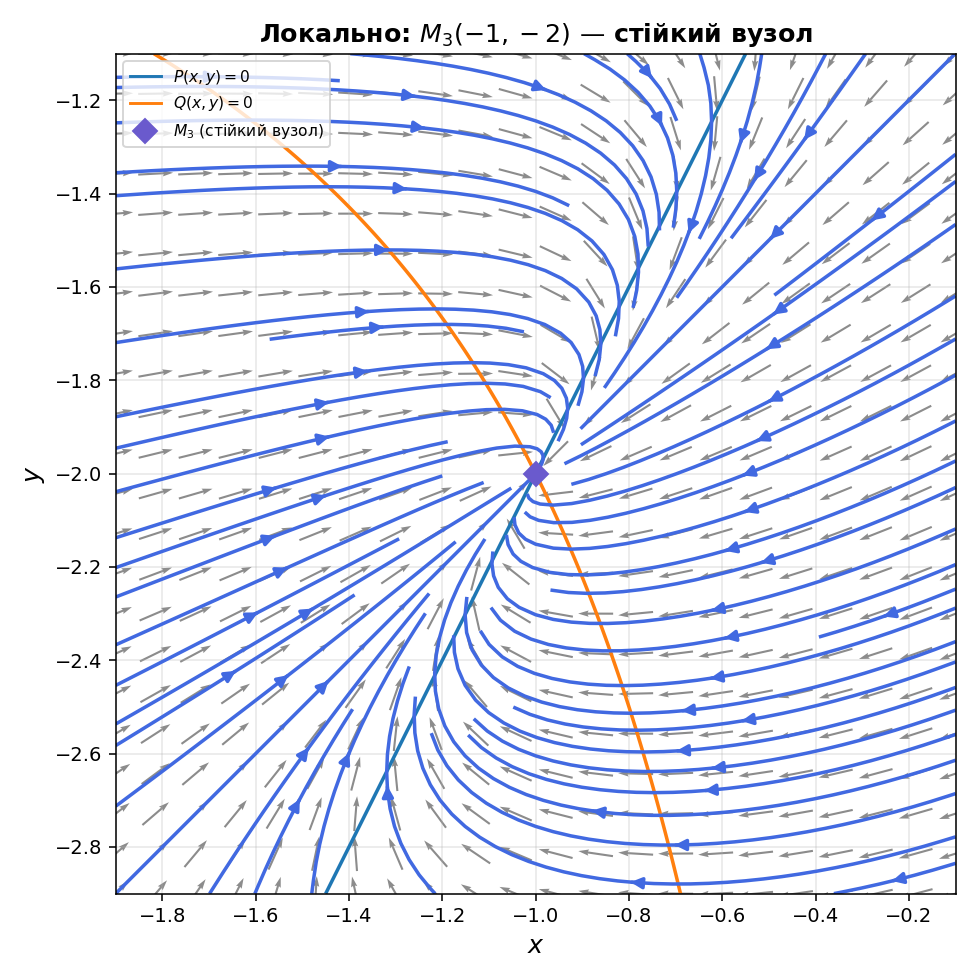
\includegraphics[width=0.72\textwidth]{local_M3.png}
    \caption{Локально біля $M_3(-1,-2)$ (стійкий вузол): траєкторії, поле напрямків та криві $\dot{x}=0$, $\dot{y}=0$}
\end{figure}

\paragraph{Код побудови (Python).}
Використовуємо ту саму універсальну функцію \texttt{plot\_local(center, tag, title)}, що й для $M_1$ (означення наведено у підрозділі про $M_1$, \textsection~\ref{subsec:M1_37}); змінюється лише точка-центр та заголовок. Оскільки $M_3$ --- вузол (не сідло), розрахунок і побудова сепаратрис не запускаються (усередині \texttt{plot\_local} є умова \texttt{if np.allclose(center, M2): saddle\_separatrices\_plot(...)}).
\begin{verbatim}
plot_local(M3, "M3",
    r"Локально: $M_3(-1,-2)$ — стійкий вузол")
\end{verbatim}

\subsection{Загальний фазовий портрет}

На рисунку~\ref{fig:global} зображено фазові траєкторії, вектори $(\dot{x},\dot{y})$ у вузлах сітки та допоміжні криві $P(x,y)=0$, $Q(x,y)=0$ на обраній області.

\begin{figure}[H]
    \centering
    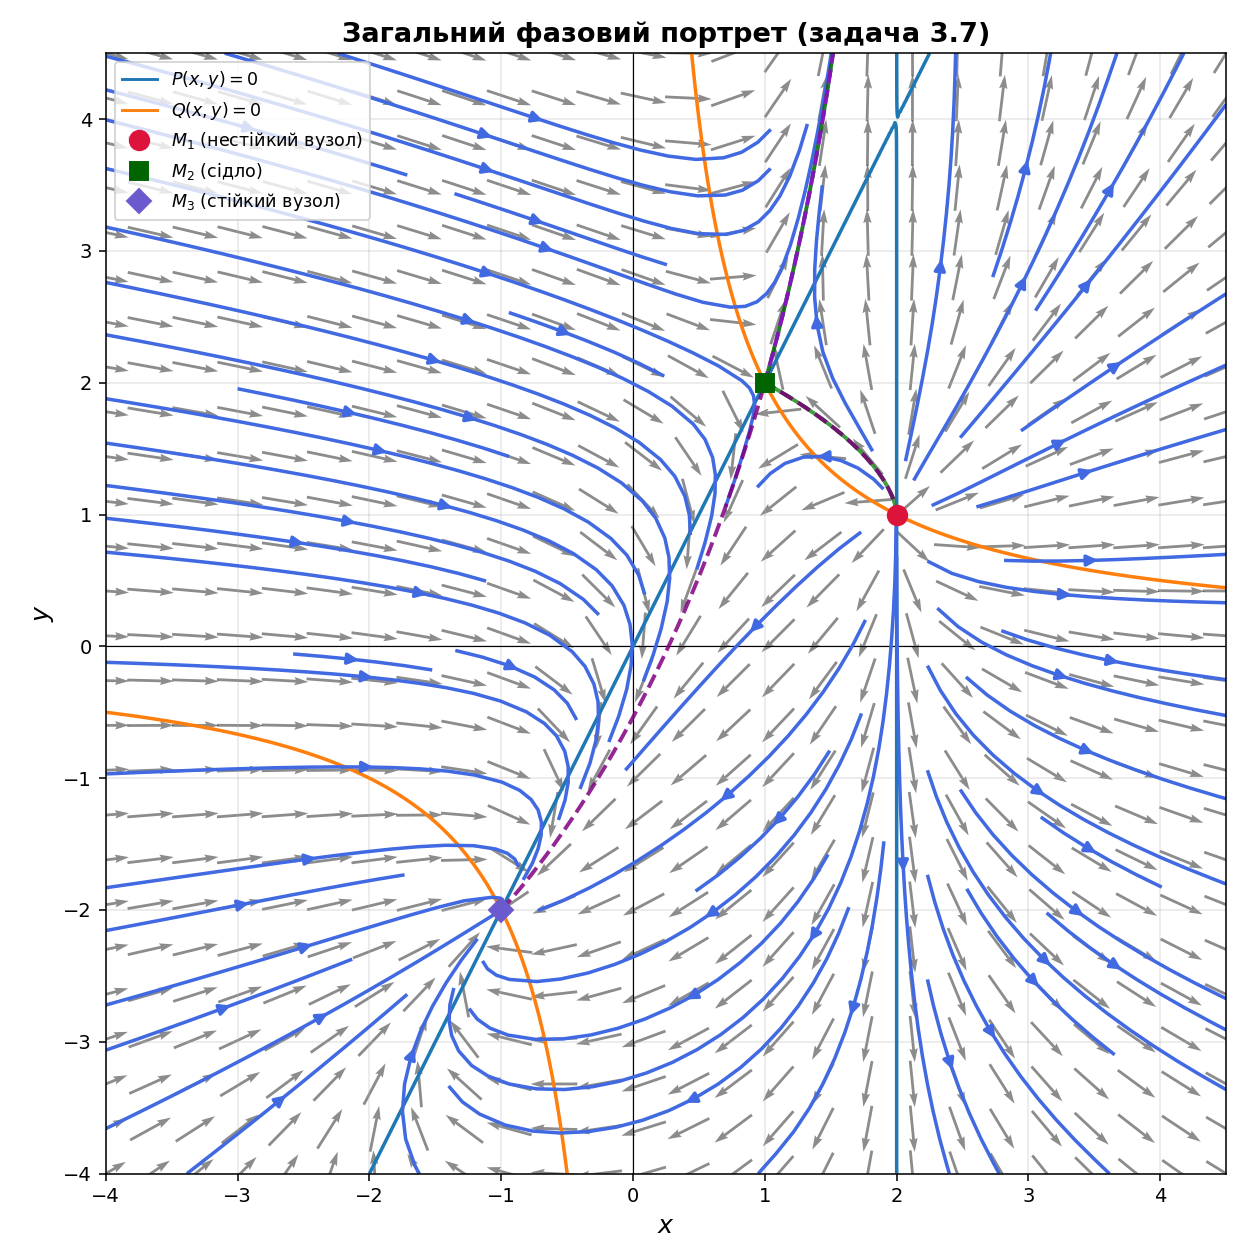
\includegraphics[width=0.82\textwidth]{global_phase_portrait.png}
    \caption{Траєкторії, поле напрямків та криві $\dot{x}=0$, $\dot{y}=0$; система~\eqref{eq:system}}
    \label{fig:global}
\end{figure}

\paragraph{Код побудови (Python).}
Функція \texttt{plot\_global()} у \texttt{phase\_portraits.py}: область по осях, \texttt{quiver}, \texttt{plot\_dx\_dy\_zero\_curves} (криві $P=0$ та $Q=0$ за \texttt{contour(..., levels=[0])}), \texttt{streamplot}, сепаратриси сідла (\texttt{saddle\_separatrices\_plot}), мітки особливих точок.
\begin{verbatim}
def plot_global():
    xlim, ylim = (-4.0, 4.5), (-4.0, 4.5)
    fig, ax = plt.subplots(figsize=(9, 9), dpi=140)
    plot_base(ax, xlim, ylim, quiver_n=26)
    plot_dx_dy_zero_curves(ax, xlim, ylim)  # dot{x}=0 та dot{y}=0
    seeds = make_seed_grid(xlim, ylim, n=10)
    stream_on_ax(ax, xlim, ylim, density=1.35, seeds=seeds)
    saddle_separatrices_plot(ax, eps=0.025, t_max=12.0)
    mark_equilibria(ax)
    fig.savefig("global_phase_portrait.png")

if __name__ == "__main__":
    plot_global()
\end{verbatim}

\subsection{Програмна реалізація (Maple)}

\begin{verbatim}
restart;
with(DEtools):
sys := {diff(x(t), t) = (2*x(t)-y(t))*(x(t)-2),
       diff(y(t), t) = x(t)*y(t)-2};
DEplot(sys, [x(t), y(t)], t = -8 .. 8, x = -4 .. 4, y = -4 .. 4,
      [[x(0)=2.5, y(0)=1.2], [x(0)=0.5, y(0)=2.5],
       [x(0)=-1.5, y(0)=-2.5]],
      arrows = MEDIUM, linecolor = blue);
\end{verbatim}

Результат побудови у Maple показано на рис.~\ref{fig:maple}.

\begin{figure}[H]
    \centering
    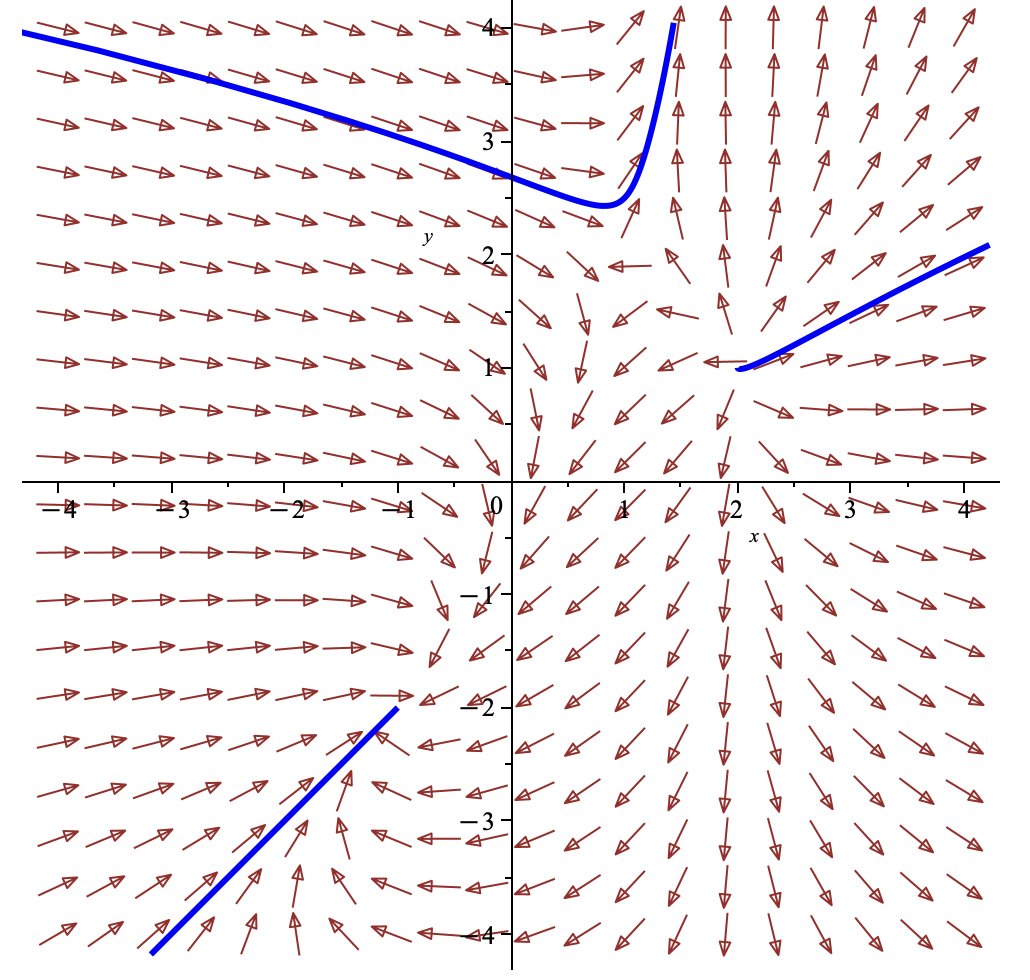
\includegraphics[width=0.85\textwidth]{maple_deplot.png}
    \caption{Поле напрямків та інтегральні криві (\texttt{DEplot}), Maple}
    \label{fig:maple}
\end{figure}

\subsection{Розширений фазовий простір}

На рис.~\ref{fig:ext37} наведено побудову у розширеному фазовому просторі $(x,y,t)$: інтегральні криві системи~\eqref{eq:system} зображено як тривимірні траєкторії, у яких вісь $t$ показує час проходження стану. Пунктирні вертикальні лінії відповідають особливим точкам $M_1$, $M_2$, $M_3$ (вони стаціонарні вздовж часу). Візуалізація виконана на Python (\texttt{plotly}, інтерактивний 3D).

\begin{figure}[H]
    \centering
    \includegraphics[width=0.95\textwidth]{\detokenize{Screenshot 2026-04-19 at 22.27.33.png}}
    \caption{Розширений фазовий простір $(x,y,t)$ для системи~\eqref{eq:system}: сітка стартових точок, інтегрована у прямому та зворотному часі (Python, \texttt{plotly})}
    \label{fig:ext37}
\end{figure}

\subsection{Висновок}

Для системи~\eqref{eq:system} знайдено три особливі точки $M_1(2,1)$, $M_2(1,2)$, $M_3(-1,-2)$.
Методом лінеаризації встановлено:
\begin{itemize}
    \item $M_1$ --- проста особлива точка типу \textbf{нестійкий вузол} ($\lambda=3,\,2$);
    \item $M_2$ --- \textbf{сідло} ($\lambda_{1,2}=\dfrac{-1\pm\sqrt{17}}{2}$);
    \item $M_3$ --- \textbf{стійкий вузол} ($\lambda=-3,\,-4$).
\end{itemize}
Усі точки прості: $\Delta(x_0,y_0)\neq 0$.
Загальний портрет на рис.~\ref{fig:global} узгоджується з локальною класифікацією та кривими $P=0$, $Q=0$.

\subsection*{Додаток: розв'язання на папері}
\addcontentsline{toc}{subsection}{Додаток: розв'язання на папері}

Нижче наведено рукописний розв'язок задачі~3.7: пошук особливих точок, розкладання в ряд Тейлора, матриця Якобі в $(x_0,y_0)$, лінеаризація в околі $M_1(2,1)$, $M_2(1,2)$, $M_3(-1,-2)$ та власні вектори.

\begin{figure}[H]
    \centering
    \includegraphics[width=0.85\textwidth]{telegram-cloud-photo-size-2-5418129556788416924-y.jpg}
    \caption{Сторінка 1: запис системи, пошук особливих точок, вивід лінеаризації через ряд Тейлора}
\end{figure}

\begin{figure}[H]
    \centering
    \includegraphics[width=0.85\textwidth]{\detokenize{2026-04-19 22.35.26.jpg}}
    \caption{Сторінка 2: слід, визначник, лінеаризована система; точка $M_1(2,1)$ --- нестійкий вузол, власні числа та власні вектори}
\end{figure}

\begin{figure}[H]
    \centering
    \includegraphics[width=0.85\textwidth]{\detokenize{2026-04-19 22.35.45.jpg}}
    \caption{Сторінка 3: точка $M_2(1,2)$ --- сідло, власні числа $\lambda_{1,2}=\tfrac{-1\pm\sqrt{17}}{2}$, власні вектори, нахили сепаратрис, перевірка напрямку}
\end{figure}

\begin{figure}[H]
    \centering
    \includegraphics[width=0.85\textwidth]{\detokenize{2026-04-19 22.35.49.jpg}}
    \caption{Сторінка 4: перевірка підстановкою у сідлі $M_2$, точка $M_3(-1,-2)$ --- стійкий вузол, власні числа $\lambda=-3,\,-4$, власні вектори, загальний розв'язок лінеаризації}
\end{figure}

\newpage
\section{Завдання 3.6}

\subsection{Запис системи}

Розглянемо автономну нелінійну систему
\begin{equation}\label{eq:system36}
\begin{cases}
\dot{x} = P(x,y) = \ln(2-y^2),\\
\dot{y} = Q(x,y) = e^{x} - e^{y}.
\end{cases}
\end{equation}
\textbf{Область визначення:} $P$ визначена за умови $2-y^2>0$, тобто
\begin{equation*}
D = \{(x,y)\in\mathbb{R}^2 : |y|<\sqrt{2}\} \quad\text{— горизонтальна смуга.}
\end{equation*}
Функція $Q$ визначена й нескінченно диференційовна на всьому $\mathbb{R}^2$; загалом $P,Q\in C^\infty(D)$.

\subsection{Знаходження особливих точок}

Особливі точки системи~\eqref{eq:system36} --- розв'язки системи
\begin{equation*}
\ln(2-y^2)=0,\qquad e^{x}-e^{y}=0.
\end{equation*}
З першого рівняння $2-y^2=1$, тобто $y^2=1$, $y=\pm 1$.
З другого, через строге зростання експоненти, $e^x=e^y \Leftrightarrow x=y$.
Звідси дві прості особливі точки:
\begin{equation*}
M_1(1,1),\qquad M_2(-1,-1).
\end{equation*}

\subsection{Матриця Якобі та інваріанти лінеаризації}

Частинні похідні:
\begin{align*}
P'_x(x,y) &= 0, &\qquad P'_y(x,y) &= \dfrac{-2y}{2-y^2},\\
Q'_x(x,y) &= e^{x}, &\qquad Q'_y(x,y) &= -e^{y}.
\end{align*}
Матриця Якобі:
\begin{equation}\label{eq:jacobian36}
J(x,y)=
\begin{pmatrix}
0 & -\dfrac{2y}{2-y^2}\\[2mm]
e^{x} & -e^{y}
\end{pmatrix}.
\end{equation}
Слід і визначник:
\begin{equation*}
\sigma(x,y)=-e^{y},\qquad
\Delta(x,y)=\det J(x,y)=0\cdot(-e^{y})-\Bigl(-\dfrac{2y}{2-y^2}\Bigr)\cdot e^{x}
=\dfrac{2y\,e^{x}}{2-y^2}.
\end{equation*}

Як і в задачі~3.7, розкладанням $P,Q$ у ряд Тейлора в околі $(x_0,y_0)$ та перенесенням $x=x_0+\xi$, $y=y_0+\eta$ отримуємо лінеаризовану систему
$\begin{pmatrix}\dot\xi\\ \dot\eta\end{pmatrix}=J(x_0,y_0)\begin{pmatrix}\xi\\ \eta\end{pmatrix}$.

\subsection{Лінеаризація в околі $M_1(1,1)$}

Підставимо $(x,y)=(1,1)$ у~\eqref{eq:jacobian36}:
\begin{equation*}
P'_y(1,1)=\dfrac{-2}{2-1}=-2,\quad Q'_x(1,1)=e,\quad Q'_y(1,1)=-e,
\end{equation*}
\begin{equation*}
J(M_1)=
\begin{pmatrix}
0 & -2\\
e & -e
\end{pmatrix}.
\end{equation*}
Маємо $\sigma(1,1)=-e$, $\Delta(1,1)=2e>0$. Характеристичне рівняння:
\begin{equation*}
\lambda^2+e\,\lambda+2e=0,\qquad D=e^2-8e=e(e-8)<0,
\end{equation*}
оскільки $e\approx 2{,}718<8$. Корені --- комплексно-спряжені:
\begin{equation*}
\lambda_{1,2}=\dfrac{-e\pm i\sqrt{\,8e-e^2\,}}{2}
=-\dfrac{e}{2}\pm i\,\dfrac{\sqrt{e(8-e)}}{2}
\approx -1{,}359\pm 1{,}895\,i.
\end{equation*}
Дійсна частина $\operatorname{Re}\lambda_{1,2}=-e/2<0$, тож $M_1$ --- \textbf{стійкий фокус}.
Оскільки $\operatorname{Re}\lambda_{1,2}\neq 0$ і $\lambda_{1,2}\neq 0$, виконана умова теореми Ляпунова про лінійне наближення: локальний портрет вихідної системи в околі $M_1$ топологічно еквівалентний спіралі лінеаризованої системи.

\paragraph{Геометрія спіралі.}
Комплексна пара $\lambda_{1,2}=-\alpha\pm i\omega$ з $\alpha=e/2\approx 1{,}359$ і $\omega=\sqrt{e(8-e)}/2\approx 1{,}895$ задає два характерні масштаби:
\begin{itemize}
    \item \emph{час згасання} $\tau=1/\alpha=2/e\approx 0{,}736$ --- за нього амплітуда радіального відхилення від $M_1$ зменшується в $e\approx 2{,}72$ рази;
    \item \emph{період обертання} $T=2\pi/\omega\approx 3{,}315$ --- час одного повного оберту навколо $M_1$.
\end{itemize}
«Тугість» спіралі визначається відношенням $\alpha/\omega=\sqrt{e/(8-e)}\approx 0{,}717$: за один оберт амплітуда змінюється у $e^{2\pi\alpha/\omega}=\exp\!\bigl(2\pi\sqrt{e/(8-e)}\bigr)\approx e^{4{,}51}\approx 90$ разів. Згасання сильне --- траєкторія практично не встигає зробити повного оберту до того, як наблизиться до $M_1$.

Напрямок обертання визначаємо підстановкою: у точці $M_1+(\varepsilon,0)$ (трохи правіше за $M_1$) маємо $\dot x=P=\ln(2-1^2)=0$, $\dot y=Q=e^{1+\varepsilon}-e\approx\varepsilon\,e>0$, тобто траєкторія в цей момент іде вгору. Отже, обертання --- \textbf{проти годинникової стрілки}.

\begin{figure}[H]
    \centering
    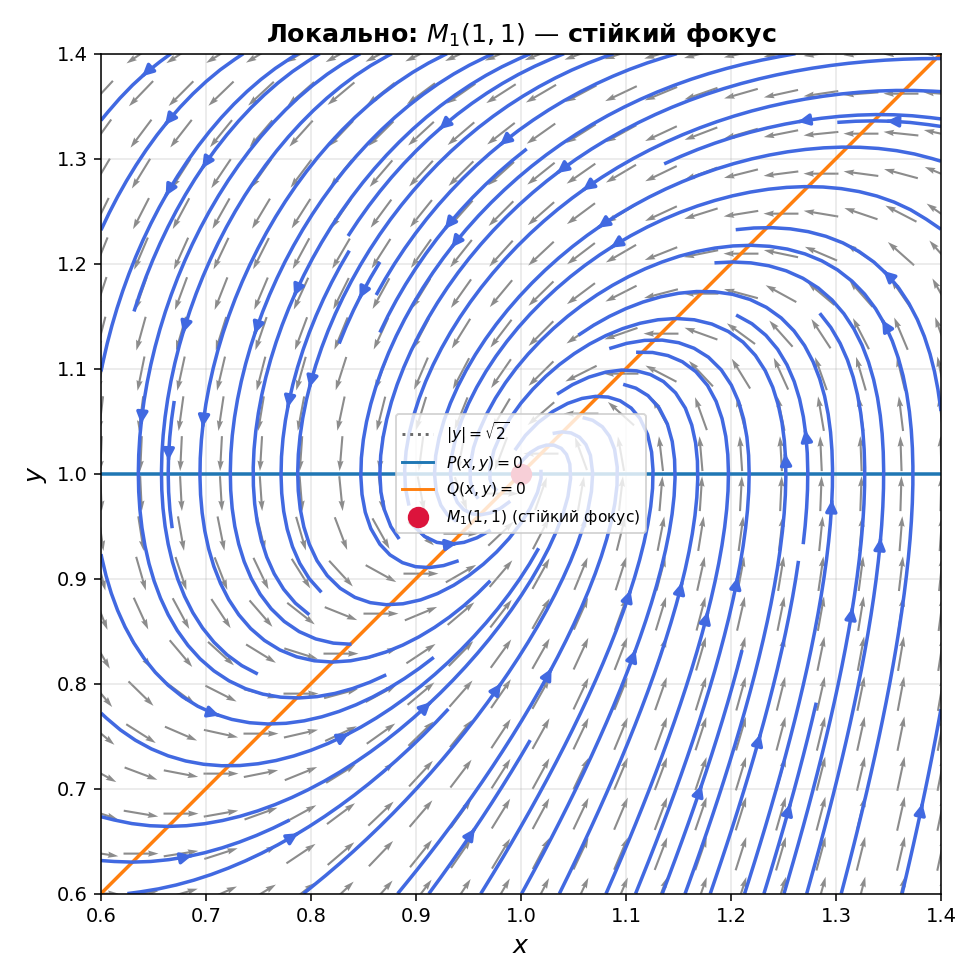
\includegraphics[width=0.65\textwidth]{local_M1_3_6.png}
    \caption{Локально біля $M_1(1,1)$ (стійкий фокус): траєкторії, поле напрямків, криві $\dot{x}=0$, $\dot{y}=0$}
\end{figure}

\paragraph{Код побудови (Python).}
\begin{verbatim}
plot_local(M1, "M1",
    r"Локально: $M_1(1,1)$ — стійкий фокус")

def P(x, y):
    arg = 2.0 - y**2
    safe = np.where(arg > 0, arg, 1.0)
    return np.where(arg > 0, np.log(safe), np.nan)

def Q(x, y):
    return np.exp(x) - np.exp(y)
\end{verbatim}

\subsection{Лінеаризація в околі $M_2(-1,-1)$}

Підставимо $(x,y)=(-1,-1)$ у~\eqref{eq:jacobian36}:
\begin{equation*}
P'_y(-1,-1)=\dfrac{-2(-1)}{2-1}=2,\quad Q'_x(-1,-1)=e^{-1},\quad Q'_y(-1,-1)=-e^{-1},
\end{equation*}
\begin{equation*}
J(M_2)=
\begin{pmatrix}
0 & 2\\
\dfrac{1}{e} & -\dfrac{1}{e}
\end{pmatrix}.
\end{equation*}
Маємо $\sigma(-1,-1)=-\dfrac{1}{e}$, $\Delta(-1,-1)=-\dfrac{2}{e}<0$, тому $M_2$ --- \textbf{сідло}. Характеристичне рівняння:
\begin{equation*}
\lambda^2+\dfrac{1}{e}\lambda-\dfrac{2}{e}=0,\qquad
\lambda_{1,2}=\dfrac{-1\pm\sqrt{\,1+8e\,}}{2e}\approx 0{,}693;\;\; -1{,}061.
\end{equation*}
Корені дійсні різних знаків, ненульові --- умова теореми Ляпунова про лінійне наближення виконана; локальний портрет вихідної системи в околі $M_2$ топологічно еквівалентний лінеаризованій системі.

Власні напрямки шукаємо у вигляді $s=(\alpha,\beta)^T$ з рівняння $(J-\lambda I)s=0$. З першого рядка $-\lambda\alpha+2\beta=0$, покладемо $\alpha=1$, тоді $\beta=\lambda/2$, тобто $s=(1,\;\lambda/2)^T$. Нахили сепаратрис лінеаризації:
\begin{equation*}
k_\pm=\dfrac{\lambda_\pm}{2}=\dfrac{-1\pm\sqrt{1+8e}}{4e}.
\end{equation*}
Напрямок руху: вздовж $s_+$ (для $\lambda_+>0$) --- від точки, вздовж $s_-$ (для $\lambda_-<0$) --- до точки.

\begin{figure}[H]
    \centering
    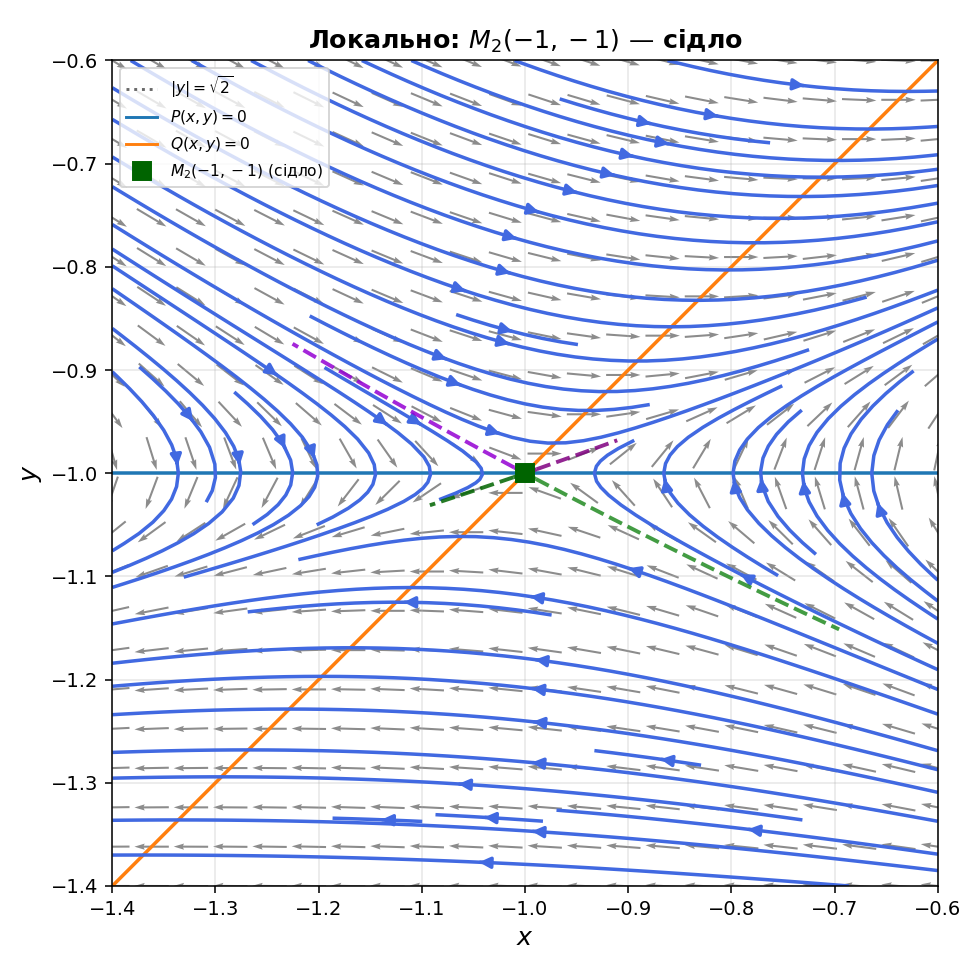
\includegraphics[width=0.65\textwidth]{local_M2_3_6.png}
    \caption{Локально біля $M_2(-1,-1)$ (сідло): траєкторії, поле напрямків, криві $\dot{x}=0$, $\dot{y}=0$ і сепаратриси}
\end{figure}

\paragraph{Код побудови (Python).}
\begin{verbatim}
J2 = np.array([[0.0, 2.0],
               [np.exp(-1.0), -np.exp(-1.0)]])
eig2, V2 = np.linalg.eig(J2)
order = np.argsort(-eig2.real)   # лямбда+ першим
v_unstable = np.real(V2[:, order[0]])
v_stable   = np.real(V2[:, order[1]])

# інтегруємо з малого зсуву вздовж власних напрямків
if np.allclose(center, M2):
    saddle_separatrices_plot(ax, eps=0.012, t_max=3.0)
\end{verbatim}

\subsection{Загальний фазовий портрет}

Оскільки функція $P(x,y)=\ln(2-y^2)$ визначена лише в смузі $|y|<\sqrt{2}$, фазовий портрет системи~\eqref{eq:system36} будуємо тільки всередині $D$; прямі $y=\pm\sqrt{2}$ позначено пунктиром як межу області означення.
Криві нульових похідних: $\dot{x}=0$ --- горизонтальні прямі $y=\pm 1$; $\dot{y}=0$ --- бісектриса $y=x$.

\begin{figure}[H]
    \centering
    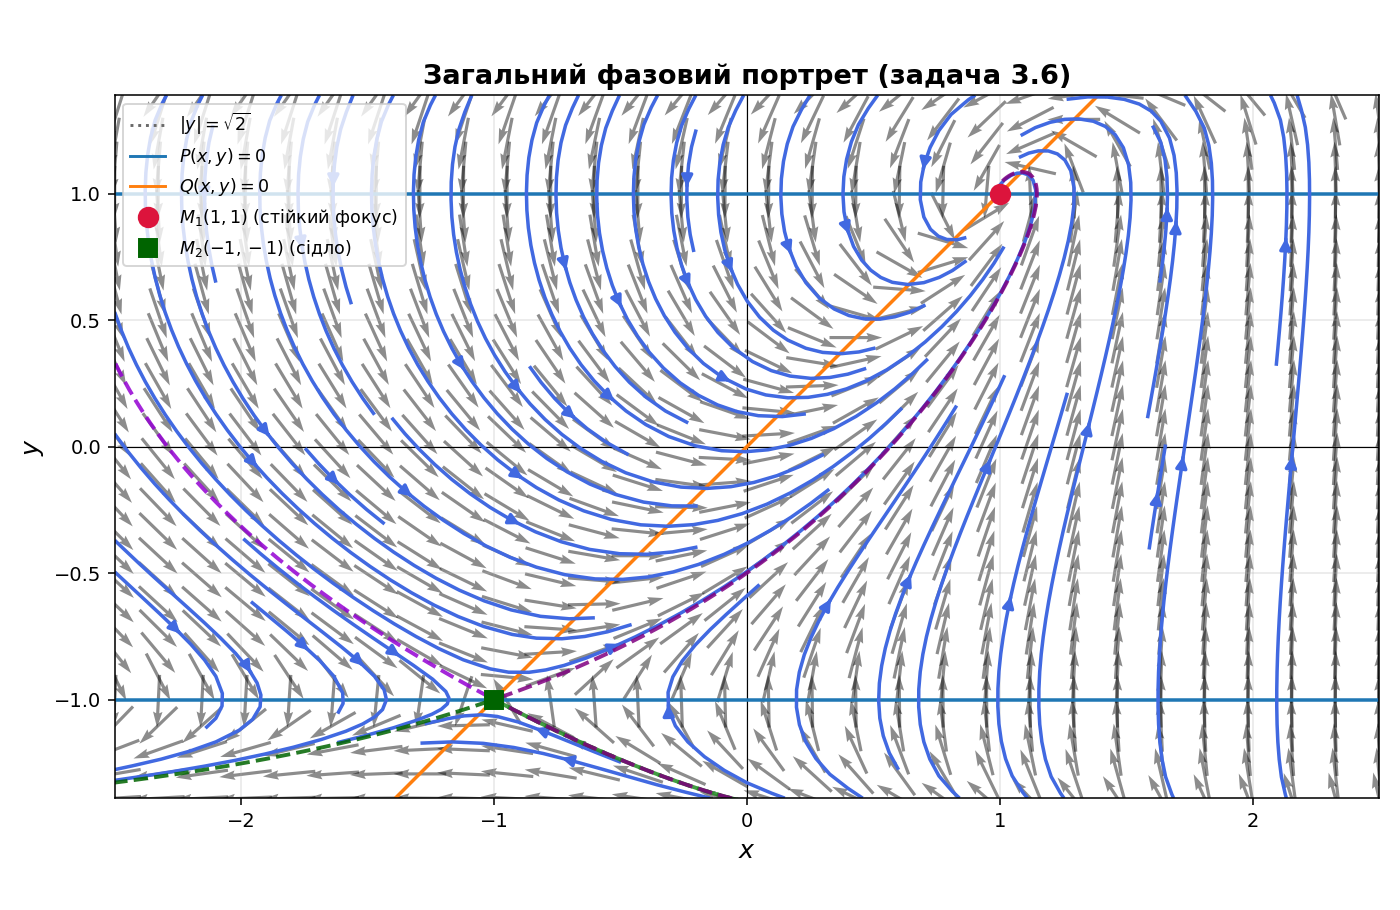
\includegraphics[width=0.9\textwidth]{global_phase_portrait_3_6.png}
    \caption{Загальний фазовий портрет системи~\eqref{eq:system36}: траєкторії, поле напрямків, криві $\dot{x}=0$, $\dot{y}=0$, сепаратриси сідла $M_2$ і межі смуги $|y|=\sqrt{2}$}
    \label{fig:global36}
\end{figure}

\paragraph{Код побудови (Python).}
\begin{verbatim}
def plot_global():
    xlim = (-2.5, 2.5); ylim = (-1.39, 1.39)
    fig, ax = plt.subplots(figsize=(10, 6.5), dpi=140)
    plot_base(ax, xlim, ylim, quiver_n=30)
    plot_domain_band(ax, xlim, ylim)          # межі |y|=sqrt(2)
    plot_dx_dy_zero_curves(ax, xlim, ylim)    # y=+-1 та y=x
    seeds = make_seed_grid(xlim, ylim, n=10,
        avoid=[(M1,0.08), (M2,0.08)])
    stream_on_ax(ax, xlim, ylim, density=1.35, seeds=seeds)
    saddle_separatrices_plot(ax, eps=0.02, t_max=10.0)
    mark_equilibria(ax)
    fig.savefig("global_phase_portrait_3_6.png")
\end{verbatim}

\subsection{Програмна реалізація (Maple)}

\begin{verbatim}
restart;
with(DEtools):
sys := {diff(x(t), t) = ln(2 - y(t)^2),
       diff(y(t), t) = exp(x(t)) - exp(y(t))};
DEplot(sys, [x(t), y(t)], t = -5 .. 5, x = -2.5 .. 2.5, y = -1.4 .. 1.4,
      [[x(0)=1.2, y(0)=0.9], [x(0)=-1.2, y(0)=-0.9],
       [x(0)=0, y(0)=0.5], [x(0)=0.5, y(0)=-0.5],
       [x(0)=1.5, y(0)=-0.6], [x(0)=-1.5, y(0)=0.6]],
      arrows = MEDIUM, linecolor = blue);
\end{verbatim}

\begin{figure}[H]
    \centering
    \includegraphics[width=0.8\textwidth]{\detokenize{Screenshot 2026-04-19 at 22.07.40.png}}
    \caption{Результат побудови фазового портрета в Maple для системи~\eqref{eq:system36}}
    \label{fig:maple36}
\end{figure}

\subsection{Розширений фазовий простір}

На рис.~\ref{fig:ext36} показано інтегральні криві системи~\eqref{eq:system36} у розширеному фазовому просторі $(x,y,t)$. Сітку стартових точок інтегровано у прямому та зворотному часі; часова вісь $t$ додає до стандартного фазового портрета інформацію про те, коли саме траєкторія проходить той чи інший стан. Пунктирні вертикальні лінії відповідають особливим точкам $M_1(1,1)$ і $M_2(-1,-1)$, а горизонтальні пунктири на площині $t=t_{\min}$ --- межі $y=\pm\sqrt{2}$ області означення. Візуалізація виконана на Python (\texttt{plotly}, інтерактивний 3D).

\begin{figure}[H]
    \centering
    \includegraphics[width=0.95\textwidth]{\detokenize{Screenshot 2026-04-19 at 22.29.02.png}}
    \caption{Розширений фазовий простір $(x,y,t)$ для системи~\eqref{eq:system36}: сітка стартових точок, межі $|y|=\sqrt{2}$ і вертикалі через $M_1,M_2$ (Python, \texttt{plotly})}
    \label{fig:ext36}
\end{figure}

\subsection{Висновок}

Для системи~\eqref{eq:system36} визначено область означення $|y|<\sqrt{2}$ та знайдено дві особливі точки:
\begin{itemize}
    \item $M_1(1,1)$ --- \textbf{стійкий фокус} ($\lambda_{1,2}=-e/2\pm i\sqrt{e(8-e)}/2$);
    \item $M_2(-1,-1)$ --- \textbf{сідло} ($\lambda_{1,2}=(-1\pm\sqrt{1+8e})/(2e)$).
\end{itemize}
Обидві точки прості: $\Delta(M_1)=2e\neq 0$, $\Delta(M_2)=-2/e\neq 0$.
Загальний фазовий портрет (рис.~\ref{fig:global36}) узгоджується з локальною класифікацією: траєкторії у смузі $|y|<\sqrt{2}$ закручуються навколо стійкого фокуса $M_1$, дві сепаратриси сідла $M_2$ поділяють область на підобласті з різною поведінкою траєкторій.

\subsection*{Додаток: розв'язання на папері}
\addcontentsline{toc}{subsection}{Додаток: розв'язання на папері (3.6)}

Нижче наведено рукописний розв'язок задачі~3.6: запис системи та області означення $|y|<\sqrt{2}$, пошук особливих точок $M_1(1,1)$, $M_2(-1,-1)$, матриця Якобі, лінеаризація в околі кожної особливої точки.

\begin{figure}[H]
    \centering
    \includegraphics[width=0.85\textwidth]{\detokenize{2026-04-19 22.37.34.jpg}}
    \caption{Сторінка 1: запис системи 3.6, область означення, пошук особливих точок, матриця Якобі та слід/визначник у $(x_0,y_0)$, перехід до лінеаризованої системи}
\end{figure}

\begin{figure}[H]
    \centering
    \includegraphics[width=0.85\textwidth,angle=90]{\detokenize{2026-04-19 22.37.38.jpg}}
    \caption{Сторінка 2: $M_1(1,1)$ --- стійкий фокус (комплексні $\lambda_{1,2}=-e/2\pm i\sqrt{e(8-e)}/2$), $M_2(-1,-1)$ --- сідло ($\lambda_{1,2}=(-1\pm\sqrt{1+8e})/(2e)$)}
\end{figure}

\end{document}
